\documentclass[11pt]{article}
\usepackage[margin=1in]{geometry}
\usepackage[T1]{fontenc}
\usepackage{lmodern}
\usepackage{amsmath,amssymb,booktabs,graphicx,microtype}
\usepackage[round,authoryear]{natbib}
\usepackage[colorlinks=true,linkcolor=blue,citecolor=blue,urlcolor=blue]{hyperref}
\usepackage{xurl}
\hypersetup{pdftitle={Judgment Gates for Paper Market Making},pdfauthor={Nicolas Coquelet}}
\newcommand{\DataDate}{2026-10-29}
\newcommand{\FramingModels}{8}
\newcommand{\FramingBudget}{28}
\newcommand{\FramingValid}{54}
\newcommand{\FramingAttempted}{74}
\newcommand{\AuditedRows}{2,645,260}
\newcommand{\AuditTime}{2026-10-30 13:25:10 UTC}
\newcommand{\ForwardAbstainOrders}{0}
\newcommand{\ForwardAbstainQuotes}{0}
\newcommand{\ForwardDecisions}{257,584}
\newcommand{\ForwardRulesSpreadBp}{0.562}
\newcommand{\ForwardClassifierSpreadBp}{0.778}
\newcommand{\ForwardFeeBp}{2.000}
\newcommand{\MarkoutCases}{96}
\newcommand{\MarkoutDayCIs}{0}
\newcommand{\MarkoutMaxDays}{1}
\newcommand{\BookComparisons}{26,525}
\newcommand{\BookErrors}{0}
\newcommand{\StateCount}{1,765}
\newcommand{\PilotCount}{443}
\newcommand{\LocalMedianUs}{2.583}
\newcommand{\LocalTailUs}{18.135}
\newcommand{\BtcRuleBrier}{0.2513}
\newcommand{\BtcClassBrier}{0.3188}
\newcommand{\WorseningMarkets}{3}
\newcommand{\MarketCount}{4}
\newcommand{\RemoteAttempts}{134}
\newcommand{\RemoteOnTime}{0}
\newcommand{\ReplayCount}{32}
\newcommand{\UnchangedReplays}{32}
\newcommand{\FrozenTrials}{698}
\newcommand{\EngineCount}{32}
\newcommand{\FrozenCommit}{12ad479abb867f03503f02632ebf93a37a161538}
\newcommand{\TestStart}{2026-10-30}
\newcommand{\TestEnd}{2027-01-28}
\newcommand{\CliGlmMedianS}{7.159}
\newcommand{\CliGlmTailS}{21.935}
\newcommand{\CliGlmSuccess}{20}
\newcommand{\CliGlmFailure}{36}
\newcommand{\GptMedianS}{16.387}
\newcommand{\GptTailS}{124.343}
\newcommand{\GptSuccess}{26}
\newcommand{\GptFailure}{5}

\title{Judgment Gates for Paper Market Making:\\A Latency-Aware Pilot and Prospective Protocol}
\author{Nicolas Coquelet\\CentraleSup\'elec \& ESSEC Business School}
\date{1 November 2026\\\small Research draft; prospective results pending}
\begin{document}
\maketitle

\begin{abstract}
Across \BookComparisons{} reconstructed-book comparisons, we observe \BookErrors{}
mismatches, and construct \StateCount{} labelled development states from Binance
and Hyperliquid BTC/ETH feeds. A logistic gate with isotonic calibration runs in
\LocalMedianUs{}~$\mu$s at the median and \LocalTailUs{}~$\mu$s at the empirical
99th percentile on Binance BTC, yet worsens Brier score on \WorseningMarkets{}
of \MarketCount{} markets; BTC changes from \BtcRuleBrier{} for rules to
\BtcClassBrier{}. The original completed remote batches produce
\RemoteOnTime{}/\RemoteAttempts{} valid answers within one second, including
failures in the denominator. Successful GLM-5.3-flash judgments through OpenCode
have median/99th-percentile client latency \CliGlmMedianS{}/\CliGlmTailS{}~s;
NVIDIA-hosted GPT-OSS-20B yields \GptMedianS{}/\GptTailS{}~s. Jev inference is
blocked by the gateway's paid-credit restriction and has no measured latency.
We provide conservative queue replay, narrow probabilistic gates, coupling and
framing protocols, and a frozen paper-only cohort. A correctness amendment leaves
all \ReplayCount{} development replay scenarios unchanged. Sparse, dependent
first-day observations do not support time-block confidence intervals, a calibrated remote
combination, or a claim of improved market-making returns. The prospective test
is registered separately and is ongoing; its final results are not evaluated.
A separate descriptive forward audit reconciles \AuditedRows{} ledger records:
the abstaining classifier submits no orders, and active variants lose after fees
and inventory effects. This monitored P\&L is not used for tuning or final inference.
The bounded framing extension returns \FramingValid{}/\FramingAttempted{} valid
judgments; only GPT-OSS and Nemotron Ultra supply paired results, with descriptive
state-bootstrap intervals rather than population invariance evidence.
\end{abstract}

\section{Introduction}
A market maker needs both a pricing rule and a decision about whether the current
state is suitable for quoting. A language model may provide contextual judgment,
but its usefulness depends on the quality, calibration and arrival time of that
judgment. A fast answer is not necessarily a useful trading signal; a probability
is not calibrated merely because an API supplies it. An emotionally neutral
interface also does not establish invariance to irrelevant framing.

We study four questions: whether route-level decision latency fits block or
second cadence; whether a local classifier and a remote model improve each other;
whether identical market features receive different answers under irrelevant
loss, win, drawdown or clock context; and whether predicted probabilities match
observed event frequencies. We keep deterministic pricing, inventory limits and
risk checks in code. Models may estimate a typed probability or a coarse regime;
they cannot generate prices or place orders.

Our contributions are an auditable first-day pilot with negative and missing
results retained; event-driven replay that charges measured decision delays and
excludes provably historical trades from queue consumption; and a prospective
protocol binding policy, source tag, continuity and ledger tail. We also provide
self-contained rescoring from committed derived receipts. These are engineering
and protocol contributions, not evidence of profitable trading or a completed
comparison of all requested models.

\section{Related work}
\citet{avellaneda2008} formulate inventory-aware quoting in a limit order book.
We use an explicitly simplified implementation as a common deterministic core.
The information component of the spread in \citet{glosten1985} motivates measuring
post-fill adverse moves, but our event label is a volatility proxy, not an
identified estimate of informed trading.

The Brier score evaluates probabilistic forecasts \citep{brier1950}.
\citet{zadrozny2002} study probability calibration from classifier scores, and
\citet{guo2017} illustrate that predictive confidence and calibration can diverge.
Neither result guarantees that isotonic calibration helps on a small, changing
crypto venue; that is measured here. Calendar-block uncertainty reflects the need
to respect dependence rather than resample individual ticks \citep{kunsch1989}.
Multiple strategy attempts also matter: the deflated Sharpe ratio addresses
selection and non-normal returns \citep{bailey2014}. We withhold its canonical
value when the dispersion across all attempted policies is unavailable.

For Jev we use Vercel's typed Decision API, with the underlying service
documented by TypeSafe \citep{typesafe,vercel}. Documentation defines an interface,
not an empirical latency or calibration result. No promotional article or social
media post supplies evidence for this study.

\section{Data}
The pilot uses public Binance USD\textcircled{\scriptsize S}-M futures and
Hyperliquid L2/trade streams for BTC and ETH, recorded on \DataDate{} (UTC). An
immutable local snapshot and its hashes are retained. The sibling recorder's
\texttt{verify} compares reconstructed books with stored top-book observations:
\BookComparisons{} comparisons pass with \BookErrors{} errors. This validates
internal reconstruction consistency, not exchange truth, queue position or
\BookComparisons{} independent predictive observations.

\begin{table}[htbp]\centering\small
\begin{tabular}{lrrrrr}
\toprule
Market & Labels & Train & Validation & Pilot & Isotonic \\
\midrule
Binance BTC & 609 & 294 & 142 & 153 & 98 \\
Binance ETH & 632 & 306 & 148 & 158 & 102 \\
Hyperliquid BTC & 301 & 144 & 71 & 76 & 48 \\
Hyperliquid ETH & 223 & 108 & 51 & 56 & 36 \\
\bottomrule
\end{tabular}

\caption{Development labels and purged chronological split counts. The isotonic
segment is inside the training period; counts need not sum across purged boundaries.}
\label{tab:data}\end{table}

Features are spread in basis points, top-five depth imbalance, signed trailing
trade flow, lagged mid return and trailing volatility. Feature computation follows
receive/processing availability and uses only previously observed events.
Let $m_t$ be the observed mid. The target is
\[
 y_t=\mathbf{1}\left\{10^4\left|\log(m_{t+10\mathrm{s}}/m_t)\right|
                 >\max(1,\mathrm{spread}_{t,\mathrm{bp}}/2)\right\}.
\]
The endpoint is the first available state at the horizon, with at most two seconds
of tolerance. Development labels reject endpoints from a different session.
Overlapping horizons and simultaneous markets make these observations dependent.
Hyperliquid's slower full-book updates are carried forward between arrivals;
the sampling grid does not create independent exchange updates. Exact historical
raw replay requires access to the retained private snapshot. Calibration and
latency were recomputed from derived receipts in the private research archive;
the public export provides aggregate statistics and precomputed paper artifacts.

\section{Method}
\subsection{Deterministic quoting and execution}
For relative-return variance $v_t$, inventory $q_t$, unit order size $s$, risk
aversion $\gamma$, horizon $T$ and arrival parameter $\kappa$, the implemented
reservation and width are
\[
 r_t=m_t[1-(q_t/s)\gamma v_tT],\qquad
 w_t=m_t\left[\gamma v_tT+\frac{2}{\gamma}\log(1+\gamma/\kappa)\right].
\]
The code rounds bids downward and asks upward using decimal tick arithmetic,
checks post-only eligibility on arrival, and enforces frozen inventory limits.
Parameters are assumptions shared by every gate, not maximum-likelihood estimates
of the venue's arrival process. Maker/taker fees are assumed to be 2/5 basis points,
respectively; no account fee schedule is claimed.

Quotes join behind displayed queue. Trades with the correct aggressor side first
consume that queue, then remaining quote size. Optimistic replay permits touching
trades; pessimistic replay requires strict traded-through prices as well as queue
consumption. Cancellation does not improve queue position. Quotes outside known
finite depth are withheld. These scenarios are sensitivity models, not proven
upper and lower bounds on actual exchange fills.

Pending cancel/replace keeps old quotes exposed until the measured judgment delay
expires; it cannot be superseded by a newer pending answer. A state older than the
registered age limit triggers a hold. Separate exchange streams can deliver old
trades after a quote has arrived. Each quote therefore records the maximum
exchange timestamp already observed at entry, from either book or trade stream.
Trades at or before this bound, or lacking an ordering timestamp, cannot consume
queue or fill. Only timestamps within the same venue clock are compared. The
bound excludes demonstrably old trades; exact exchange order-entry time between
observations remains unobserved.

\subsection{Gates, coupling and abstention}
Rules and a standardised logistic classifier use identical numeric features.
Logistic regularisation is fixed; isotonic calibration uses a later, purged part
of training. Expanding chronological folds provide development diagnostics.
Abstention thresholds minimise validation Brier loss with a fixed rejection cost;
rejected states do not submit quotes. A zero-profit, zero-coverage policy is not
interpreted as a superior market maker.

Remote clients use the same market features for narrow typed judgments.
Jev asks a Boolean veto through \path{/v1/evaluate}; its probability is the
shared toxicity-proxy target. It uses no chat messages; thresholds, prices and
risk remain in code. The older TypeSafe-compatible access probe is retained as
historical evidence. A fresh cheap decision preflight precedes the resumable
calibration, framing and coupling command. The
registered targets include Jev, GLM-5.3-flash, DeepSeek-v4.1-flash and GPT-OSS, with
a large model restricted to minute-cadence regime judgments. Client time includes
transport, queueing, retries and, for OpenCode, CLI startup; shared NIM-slot waiting
is excluded. Retries and failures are retained. Cached response reuse is not a new
physical latency measurement. Historical aliases do not reveal immutable served
model revisions.

A validation-fitted stack forms $p=wp_C+(1-w)p_R$. An uncertainty cascade calls
the remote gate only inside a validation-selected classifier uncertainty band;
its replay charges both local and remote delay on those decisions. A combined
confidence threshold permits abstention. Neither fitted weights nor financial
outcomes are reported without a complete common validation/pilot prediction
matrix. The large-model regime mask also honours the arrival time of each update.

\subsection{Calibration and framing}
We report $\mathrm{Brier}=n^{-1}\sum_i(p_i-y_i)^2$, equal-width reliability bins,
and $\mathrm{ECE}=\sum_b(n_b/n)|\bar p_b-\bar y_b|$. ECE depends on binning and
sample size; isotonic levels can be few. Framing tests keep market features fixed
and vary only irrelevant recent P\&L, drawdown wording or clock context. A neutral
repeat measures generation variability. We measure signed/absolute probability
shifts and decision flips. Local numeric gates are deterministic, with no prompt
state; this is an implementation property, not psychological evidence.
Alongside the UTC-block analysis, a review-requested descriptive bootstrap
resamples paired market-state differences (2,000 draws, seed 42, percentile 95\%
intervals, at least two pairs). These post-hoc development intervals assume
exchangeable pairs, have no multiplicity adjustment and do not establish
independent-day precision. Neutral repeats retain generation variability.

\section{Protocol}
The split is chronological: the first half trains, the next quarter validates,
and the last quarter is an exploratory pilot. Full label horizons are purged at
boundaries. Calibration uses a purged internal training segment, with scaling fit
on training only. Repeated experiments on this pilot remain development; they
are not repeated held-out tests. No seed is selected for a favourable outcome.

The ongoing prospective local cohort is \texttt{forward-v4}, from \TestStart{} inclusive
to \TestEnd{} exclusive in UTC. Its \EngineCount{} engines span rules/classifier,
with/without abstention, and both fill scenarios across all markets. Numerical
coefficients, cutoffs and limits remain fixed. Earlier commissioning tags were
withdrawn for decimal queue lookup, finite-depth handling and finally ordering/
scoring defects; their histories and losses remain available. The review
amendment leaves \UnchangedReplays{}/\ReplayCount{} development executions unchanged.
Remote gates are excluded from this local cohort and need a separate future
registration if access and validation predictions become adequate.

The primary family contains the pessimistic, non-abstaining classifier-minus-rules
10-second markout comparison in each market. We compare equal-weight matched-hour
means, not unrelated individual fills. UTC hour/day block resampling uses 2,000
replicates and seed 42. The primary family uses Bonferroni $\alpha=0.05/4$; optimistic
comparisons and other intervals are labelled descriptive. Fewer than five blocks
yields no CI. The one-basis-point half-width target additionally requires five
complete days with at least 90\% decision coverage. Coverage enumerates missing
engines and boundary hours. Annualised risk ratios require a pre-window P\&L
baseline, boundary observations and 90\% coverage in every registered hour, as
well as adequate variable hourly returns; missing hours are never compressed.

The frozen pre-test register counts \FrozenTrials{} variants/iterations
conservatively, including correlated attempts. All-trial Sharpe dispersion is
unavailable. Canonical DSR is therefore null; retained-variant sensitivity is
explicitly separate and is also not estimable in this short pilot. No all-trial
DSR significance claim is made.

Prospective decisions and fills carry continuity identities. Explicit gaps,
process starts and session changes censor pending labels and markouts; horizon-end
and endpoint-tolerance censoring are reported separately. A label never bridges
a known outage. The final scorer checks policy bytes against its immutable Git
tag, validates every start identity and verifies the complete hash chain through
a captured checkpoint tail. Scoring is reserved by cohort identity, independently
of output filename. This assumes the cohort directory and local anchors are
trusted; it does not defeat an attacker replacing all anchors or copying the
cohort to bypass a local reservation. No final test has been evaluated. A separate bounded framing extension fixes
\FramingModels{} named NIM models and at most \FramingBudget{} judgments per model
on four evenly spaced original development states and all framing contexts.
It uses the shared two-slot mutex, sequential requests, a 30-second read timeout,
no timeout retries, backoff on rate/server errors and a three-failure cutoff.
It neither tunes a financial policy nor adds rows to the frozen prospective cohort.

\section{Results}
\subsection{Calibration: a fast local gate can be worse}
\begin{table}[htbp]\centering\small
\begin{tabular}{lrrrrr}
\toprule
Market & $n$ & Brier R & Brier C & ECE R & ECE C \\
\midrule
Binance BTC & 153 & 0.2513 & 0.3188 & 0.2482 & 0.3371 \\
Binance ETH & 158 & 0.2520 & 0.3802 & 0.0945 & 0.3631 \\
Hyperliquid BTC & 76 & 0.1791 & 0.1671 & 0.1405 & 0.0908 \\
Hyperliquid ETH & 56 & 0.2436 & 0.3347 & 0.1914 & 0.3123 \\
\bottomrule
\end{tabular}

\caption{Exploratory local calibration on identical per-market pilot labels.
R denotes rules; C denotes logistic plus isotonic calibration. Lower is better.}
\label{tab:calibration}\end{table}
Table~\ref{tab:calibration} reports all markets. The classifier worsens Brier on
\WorseningMarkets{} of \MarketCount{} markets. Its Binance BTC score rises from
\BtcRuleBrier{} to \BtcClassBrier{} despite very fast inference. Figure~\ref{fig:reliability}
shows bin-level behaviour; neither sparsely occupied bins nor a few isotonic
levels justify an assertion of reliable confidence. The pilot is too short for
the registered block CIs.

\begin{table}[htbp]\centering\small
\begin{tabular}{lrrrr}
\toprule
Market & $n$ & $\Delta$ Brier (C--R) & UTC hours & Block 95\% CI \\
\midrule
Binance BTC & 153 & 0.0675 & 1 & -- \\
Binance ETH & 158 & 0.1283 & 1 & -- \\
Hyperliquid BTC & 76 & -0.0120 & 1 & -- \\
Hyperliquid ETH & 56 & 0.0911 & 1 & -- \\
\bottomrule
\end{tabular}

\caption{Paired classifier-minus-rules Brier differences on existing development
labels. Positive is worse for the classifier. Each market occupies one UTC hour;
the minimum independent-block requirement is unmet, so intervals remain absent.}
\label{tab:uncertainty}\end{table}
Table~\ref{tab:uncertainty} retains paired differences rather than treating
overlapping labels as independent observations. Across \MarkoutCases{} development
markout cases (all gates, fill scenarios and horizons), \MarkoutDayCIs{} support a
day-block CI, with at most \MarkoutMaxDays{} UTC day represented. No one-basis-point
test precision claim follows. More bootstrap draws cannot replace observed days;
the prospective final scorer remains reserved until its registered end.

\begin{figure}[htbp]\centering
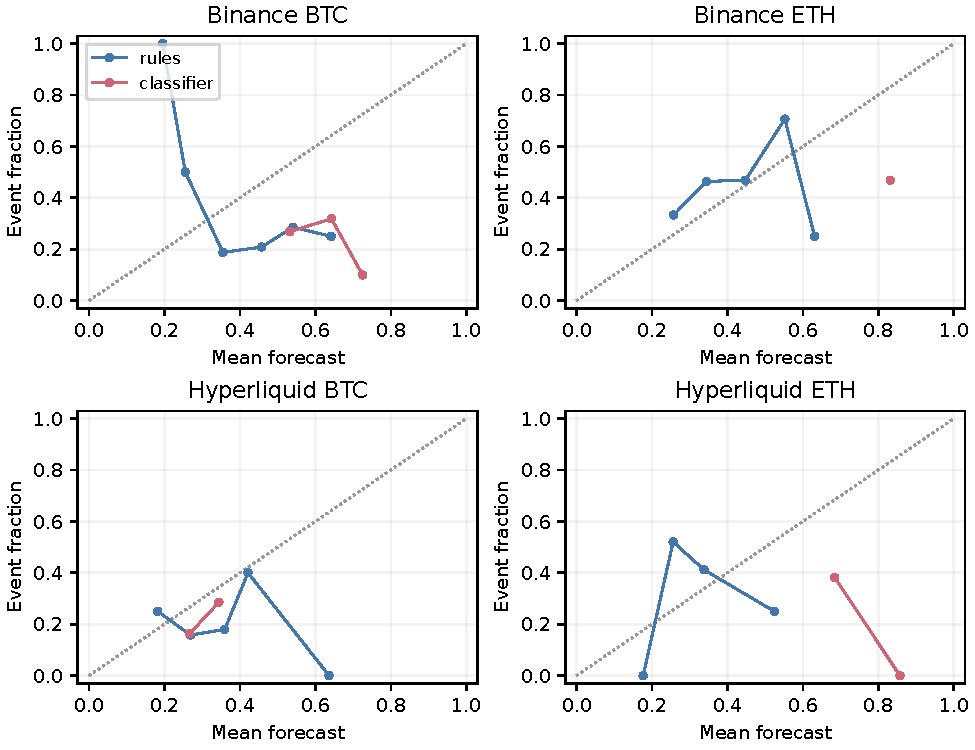
\includegraphics[width=.92\linewidth]{generated/reliability.pdf}
\caption{Reliability diagrams generated from committed pilot receipts. Lines
join occupied bins for readability; they are not fitted calibration functions.
There are no confidence bands because the independent-block requirement is unmet.}
\label{fig:reliability}\end{figure}

\subsection{Latency: measured routes do not support subsecond judgment}
\begin{table}[htbp]\centering\small
\begin{tabular}{lrrrr}
\toprule
Model / route & Valid & Failed & p50 (s) & p99 (s) \\
\midrule
GLM-5.3-flash / CLI & 20 & 36 & 7.159 & 21.935 \\
DeepSeek-v4.1-flash / CLI & 0 & 30 & -- & -- \\
GLM-5.3-flash / NIM & 0 & 3 & -- & -- \\
DeepSeek-v4.1-flash / NIM & 0 & 3 & -- & -- \\
GPT-OSS-20B / NIM & 26 & 5 & 16.387 & 124.343 \\
Nemotron Ultra / NIM & 5 & 4 & 32.265 & 51.029 \\
Jev / Gateway & not run & access 403 & -- & -- \\
\bottomrule
\end{tabular}

\caption{Original completed remote batches. Quantiles condition on valid answers
and are unstable at these sample sizes. Failed judgments retain retries/timeouts.
Jev access rejection is not an inference failure or latency sample.}
\label{tab:remote}\end{table}
The stored Binance BTC local benchmark gives \LocalMedianUs{}/\LocalTailUs{}~$\mu$s
for classifier p50/p99. Table~\ref{tab:remote} reports the remote routes separately.
The original batches and the explicit CLI quota recheck achieve
\RemoteOnTime{}/\RemoteAttempts{} valid judgments within one second; all failures
remain in the denominator. These are route/configuration-specific observations,
not universal lower bounds on model speed. Figure~\ref{fig:latency} includes
failures in its denominator rather than plotting only successful latency CDFs.
It excludes the separate quota recheck, whose failures are counted in the deadline
receipt, and does not pool configurations.

\begin{figure}[htbp]\centering
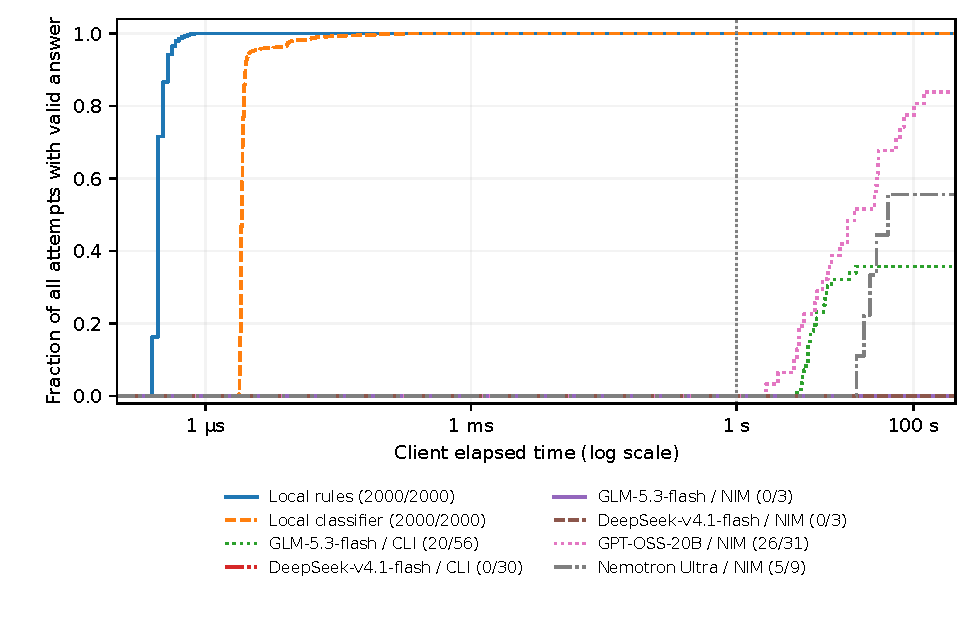
\includegraphics[width=\linewidth]{generated/latency.pdf}
\caption{Valid-answer arrival fractions in the original batches; legend counts
are valid/all attempts. NIM resource-slot waiting is excluded; CLI startup and
request retries are included. Zero-success curves overlap at zero. Jev has no
inference curve. No confidence band is supported.}
\label{fig:latency}\end{figure}

NIM flash judgments time out in the tested configuration; this does not establish
that the models themselves cannot answer quickly. The original Nemotron run has
both valid answers and truncated reasoning outputs. A later budget configuration
returns HTTP 400 on every attempted request and cannot supply a regime replay.
Jev's documented gateway route returns an account paid-credit restriction despite
positive promotional credit; no native key exists. We measure neither native Jev
nor gateway inference latency. Gateway rejection time is not substituted for it.
Cost per million operational decisions is unmeasured: free/trial access and token
catalogue prices cannot establish production unit cost, failure cost or coverage.

\subsection{Execution: sparse fills and no established economic gain}
\begin{table}[htbp]\centering\small
\begin{tabular}{lrrrrr}
\toprule
Market / gate & Fills & Spread (\$) & Inventory (\$) & Fees (\$) & P\&L (\$) \\
\midrule
Binance BTC / R & 4 & 0.00370 & -0.08860 & 0.06415 & -0.14905 \\
Binance BTC / R+A & 1 & 0.00805 & -0.02570 & 0.01604 & -0.03369 \\
Binance BTC / C & 0 & 0.00000 & 0.00000 & 0.00000 & 0.00000 \\
Binance BTC / C+A & 0 & 0.00000 & 0.00000 & 0.00000 & 0.00000 \\
Binance ETH / R & 1 & 0.00085 & 0.00300 & 0.00464 & -0.00079 \\
Binance ETH / R+A & 0 & 0.00000 & 0.00000 & 0.00000 & 0.00000 \\
Binance ETH / C & 0 & 0.00000 & 0.00000 & 0.00000 & 0.00000 \\
Binance ETH / C+A & 0 & 0.00000 & 0.00000 & 0.00000 & 0.00000 \\
Hyperliquid BTC / R & 0 & 0.00000 & 0.00000 & 0.00000 & 0.00000 \\
Hyperliquid BTC / R+A & 0 & 0.00000 & 0.00000 & 0.00000 & 0.00000 \\
Hyperliquid BTC / C & 0 & 0.00000 & 0.00000 & 0.00000 & 0.00000 \\
Hyperliquid BTC / C+A & 0 & 0.00000 & 0.00000 & 0.00000 & 0.00000 \\
Hyperliquid ETH / R & 0 & 0.00000 & 0.00000 & 0.00000 & 0.00000 \\
Hyperliquid ETH / R+A & 0 & 0.00000 & 0.00000 & 0.00000 & 0.00000 \\
Hyperliquid ETH / C & 0 & 0.00000 & 0.00000 & 0.00000 & 0.00000 \\
Hyperliquid ETH / C+A & 0 & 0.00000 & 0.00000 & 0.00000 & 0.00000 \\
\bottomrule
\end{tabular}

\caption{All pessimistic development scenarios, in USD. R/C denote rules/classifier;
+A adds validation-selected abstention. Inventory is the marked inventory component;
spread plus inventory minus fees reconciles P\&L. Zero fills are retained.}
\label{tab:pnl}\end{table}
\begin{table}[htbp]\centering\small
\begin{tabular}{lrrrr}
\toprule
Market / gate & Fill rate & 1 s bp ($n$) & 10 s bp ($n$) & 60 s bp ($n$) \\
\midrule
Binance BTC / R & 0.0208 & -0.158 (3) & -0.249 (3) & -0.349 (1) \\
Binance BTC / C & 0.0000 & -- (0) & -- (0) & -- (0) \\
Binance ETH / R & 0.0036 & -1.034 (1) & -- (0) & -- (0) \\
Binance ETH / C & 0.0000 & -- (0) & -- (0) & -- (0) \\
Hyperliquid BTC / R & 0.0000 & -- (0) & -- (0) & -- (0) \\
Hyperliquid BTC / C & 0.0000 & -- (0) & -- (0) & -- (0) \\
Hyperliquid ETH / R & 0.0000 & -- (0) & -- (0) & -- (0) \\
Hyperliquid ETH / C & 0.0000 & -- (0) & -- (0) & -- (0) \\
\bottomrule
\end{tabular}

\caption{Pessimistic non-abstaining development diagnostics. Markout cells show
mean signed mid move in bp and usable endpoint count; missing endpoints are
censored. Fill rate is filled volume/submitted volume. No block CI is supported.}
\label{tab:markouts}\end{table}
Fees, inventory and adverse mid moves can dominate a small captured spread.
Tables~\ref{tab:pnl}--\ref{tab:markouts} make low activity and missing markouts
visible. A post-fill markout overlaps inventory P\&L and is not added a second
time to the cash decomposition. Optimistic results, hypothetical taker flattening
and complete fill/equity records remain in the receipts. The pilot cannot support
annualised Sharpe/Sortino or a deflated performance conclusion. It has not shown
that a faster gate, classifier, or abstention improves economically meaningful
market-making outcomes.

\subsection{Provisional forward activity and fee drag}
\begin{table}[htbp]\centering\small
\begin{tabular}{lrrrrr}
\toprule
Gate / scenario & Fills & Spread (\$) & Fees (\$) & Inventory (\$) & P\&L (\$) \\
\midrule
C+A / opt. & 0 & 0.00 & 0.00 & 0.00 & 0.00 \\
C+A / pess. & 0 & 0.00 & 0.00 & 0.00 & 0.00 \\
C / opt. & 7165 & 32.44 & 82.58 & -145.54 & -195.68 \\
C / pess. & 6714 & 30.47 & 78.31 & -143.00 & -190.84 \\
R+A / opt. & 693 & 3.15 & 9.58 & -20.46 & -26.88 \\
R+A / pess. & 663 & 2.94 & 9.19 & -24.31 & -30.56 \\
R / opt. & 19330 & 53.56 & 182.55 & -236.12 & -365.11 \\
R / pess. & 18257 & 49.43 & 175.81 & -230.37 & -356.75 \\
\bottomrule
\end{tabular}

\caption{Descriptive cumulative paper monitoring through \AuditTime{}, aggregated
across markets from commissioning, including time before the test window.
R/C denote rules/classifier, +A denotes abstention. The audited prefix contains
\AuditedRows{} records. Both fill scenarios are retained; these are not final test
results or confidence estimates.}
\label{tab:forward}\end{table}
The read-only audit verifies the full checkpoint hash chain and reconstructs fill
cash and inventory independently before reconciling each engine's latest mark.
Table~\ref{tab:forward} never sums cumulative balances across days.
The abstaining classifier submits \ForwardAbstainOrders{} orders and has
\ForwardAbstainQuotes{} quote-present observations across \ForwardDecisions{}
decisions per fill scenario. Its zero P\&L is inactivity. The no-abstention variants
retain toxicity vetoes, stale-state holds and hard risk limits; they are not
unconditional quoting policies.

In the pessimistic scenario, rules and classifier capture respectively
\ForwardRulesSpreadBp{} and \ForwardClassifierSpreadBp{} basis points of filled
notional, below the assumed \ForwardFeeBp{} basis point maker fee. Spread capture
thus fails to cover fees even before inventory losses. The inventory column is
the residual that reconciles marked P\&L to fill-mid spread capture minus fees;
markouts overlap it and must not be added again. The frozen pricing core lacks a
fee-aware minimum spread, so the losses do not isolate gate quality. Monitoring
does not trigger policy retuning or an early held-out significance claim.

\subsection{Framing and remote calibration remain underpowered}
\begin{table}[htbp]\centering\footnotesize
\begin{tabular}{lrrrr}
\toprule
Model / route & $n_D$ & Drawdown [95\% CI] & $n_R$ & Repeat [95\% CI] \\
\midrule
GLM-5.3-flash / CLI & 2 & 0.440 [-0.020, 0.900] & 2 & 0.015 [0.010, 0.020] \\
GPT-OSS-20B / NIM & 4 & -0.327 [-0.795, 0.141] & 4 & -0.217 [-0.727, 0.075] \\
Nemotron Ultra / NIM & 1 & 0.130 [--] & 1 & 0.000 [--] \\
\bottomrule
\end{tabular}

\caption{Paired signed probability shifts relative to neutral framing. Neutral
repeat is a separate fresh generation on the same features. Brackets show
descriptive paired-state bootstrap intervals, not UTC-block intervals; small $n$
is not evidence of invariance. A dash denotes fewer than two state pairs.}
\label{tab:tilt}\end{table}
\begin{table}[htbp]\centering\small
\begin{tabular}{lrrr}
\toprule
Model / route & $n$ & Brier & ECE \\
\midrule
GLM-5.3-flash / CLI & 3 & 0.0063 & 0.0733 \\
GPT-OSS-20B / NIM & 4 & 0.5813 & 0.6455 \\
Nemotron Ultra / NIM & 1 & 0.9604 & 0.9800 \\
\bottomrule
\end{tabular}

\caption{Sparse neutral remote calibration diagnostics. These use different tiny
state subsets from the full local pilot and cannot rank models against each other.}
\label{tab:remotecal}\end{table}
Table~\ref{tab:tilt} shows that irrelevant drawdown wording can coincide with large
probability shifts, while a neutral repeat can also shift. The sample cannot
reliably separate framing susceptibility from stochastic generation. Local rules
and classifier are invariant because distractors never enter their numeric
features. Jev and the unavailable flash route have no paired inference result
in the original batches.
Table~\ref{tab:remotecal} is a diagnostic rather than evidence of transferable
calibration.

\ifnum\FramingAttempted>0
\begin{table}[htbp]\centering\scriptsize
\begin{tabular}{lrrrrr}
\toprule
NIM model & Valid/tried & $n_D$ & Drawdown [95\% CI] & $n_R$ & Repeat [95\% CI] \\
\midrule
GLM-5.3-flash & 0/3 & 0 & -- [--] & 0 & -- [--] \\
GLM-5.3 & 0/3 & 0 & -- [--] & 0 & -- [--] \\
DeepSeek-v4.1-flash & 0/3 & 0 & -- [--] & 0 & -- [--] \\
Gemma-4-31B-it & 0/3 & 0 & -- [--] & 0 & -- [--] \\
MiniMax-M3.1-flash & 0/3 & 0 & -- [--] & 0 & -- [--] \\
Nemotron Lightning & 0/3 & 0 & -- [--] & 0 & -- [--] \\
Nemotron Ultra & 27/28 & 3 & 0.0167 [-0.0300, 0.0800] & 3 & -0.0100 [-0.0500, 0.0200] \\
GPT-OSS-20B & 27/28 & 4 & 0.2328 [0.0000, 0.4655] & 4 & 0.0625 [-0.0050, 0.1300] \\
\bottomrule
\end{tabular}

\caption{Bounded review framing extension, separate from the original batches.
Valid/tried counts judgments; $n_D,n_R$ count complete drawdown/neutral-repeat
pairs. Brackets are descriptive paired-state bootstrap intervals; missing pairs
are retained. No independent-day precision or model ranking is established.}
\label{tab:extension}\end{table}

The extension returns \FramingValid{}/\FramingAttempted{} valid judgments.
Table~\ref{tab:extension} includes every prespecified model, including failed or
incomplete routes; it does not pool configurations into the original latency
headline.

Only GPT-OSS-20B and Nemotron Ultra produce valid answers. Each has one timeout;
GLM-5.3 returns HTTP 410, Nemotron Lightning returns unparseable answers, and
the remaining routes time out. Failed judgments have no probability or framing
interval and are not treated as invariant responses.

\begin{table}[htbp]\centering\scriptsize
\begin{tabular}{lrrrr}
\toprule
NIM model & Context & $n$ & Shift [95\% CI] & Flip fraction [95\% CI] \\
\midrule
Nemotron Ultra & loss & 3 & 0.0100 [0.0000, 0.0300] & 0.0000 [0.0000, 0.0000] \\
Nemotron Ultra & win & 3 & 0.0133 [0.0100, 0.0200] & 0.0000 [0.0000, 0.0000] \\
Nemotron Ultra & drawdown & 3 & 0.0167 [-0.0300, 0.0800] & 0.0000 [0.0000, 0.0000] \\
Nemotron Ultra & morning & 3 & -0.1030 [-0.3290, 0.0200] & 0.0000 [0.0000, 0.0000] \\
Nemotron Ultra & night & 3 & 0.0100 [-0.0300, 0.0700] & 0.0000 [0.0000, 0.0000] \\
Nemotron Ultra & neutral repeat & 3 & -0.0100 [-0.0500, 0.0200] & 0.0000 [0.0000, 0.0000] \\
GPT-OSS-20B & loss & 4 & 0.1859 [-0.0003, 0.5580] & 0.2500 [0.0000, 0.7500] \\
GPT-OSS-20B & win & 4 & 0.0996 [-0.0004, 0.2992] & 0.0000 [0.0000, 0.0000] \\
GPT-OSS-20B & drawdown & 4 & 0.2328 [0.0000, 0.4655] & 0.2500 [0.0000, 0.7500] \\
GPT-OSS-20B & morning & 4 & 0.1190 [0.0000, 0.3570] & 0.0000 [0.0000, 0.0000] \\
GPT-OSS-20B & night & 3 & 0.1069 [0.0000, 0.3200] & 0.0000 [0.0000, 0.0000] \\
GPT-OSS-20B & neutral repeat & 4 & 0.0625 [-0.0050, 0.1300] & 0.0000 [0.0000, 0.0000] \\
\bottomrule
\end{tabular}

\caption{Every non-neutral framing condition in the completed extension for
models with valid pairs. Shifts are signed probability differences from neutral;
flip fractions compare thresholded decisions. Brackets are unadjusted descriptive
paired-state bootstrap intervals. Degenerate zero-flip intervals do not establish
population invariance; independent time-block CIs remain unavailable.}
\label{tab:contexts}\end{table}

GPT-OSS's drawdown interval touches zero; Nemotron Ultra's contains zero.
Nemotron's small win-context shift has an interval excluding zero, but this is a
tiny conditional cohort with no multiple-testing correction. Neutral repeats also
vary. Table~\ref{tab:contexts} retains all tested contexts, rather than selecting
only the largest shift. These observations cannot establish an emotion-free gate
or separate framing effects from generation variability reliably.
\else
The bounded framing extension remains queued behind occupied shared NIM slots;
no request from that extension has been attempted at this checkpoint. No
inference outcome or invariance conclusion is inferred from waiting.
\fi
Complete common predictions are absent, so stacks, cascades and
remote abstention variants remain not run rather than being fitted to a convenient
subset. Q1 has preliminary route measurements; Q2 remains untested; Q3 and Q4
have only limited development evidence. None has a well-powered population answer.

\section{Limitations}
The main limitation is observation time: overlapping samples from a first-day
pilot do not establish precision across days or regimes. Small isotonic segments,
a volatility-proxy label and repeated pilot inspection further limit generality.
Providers, prompts, quotas, failure cutoffs and timing routes differ. Empirical
p99 from a handful of successes does not estimate a reliable service-level tail;
resource contention and client overhead can matter. Neither vendor latency nor
vendor calibration claims are tested without valid Jev inference.

L2 aggregation hides individual queue priorities, hidden orders, cancellations,
RPI liquidity and own market impact. Hypothetical fees omit funding and any
account-specific discounts. Kill-on-gap is idealised: real cancellations could
arrive late and unseen fills could occur. Source-time bounds leave uncertain
ordering between observations. A laptop can suspend or disconnect despite
launchd and idle-sleep inhibition; commissioning health proves neither uninterrupted
operation nor future uptime. The full requested remote forward matrix and
multi-month acceptance remain incomplete.

The private history includes hosted outputs and exchange-derived rows. Weight
licences do not establish redistribution permission. The public export includes
original code, synthetic tests, this paper and author-computed aggregate statistics;
underlying market observations, provider responses and private history are excluded.
There is no claim of a publicly available historical raw archive or of an arXiv
submission. These access limitations reduce independent empirical reproducibility.

\section{Reproducibility}
The frozen runtime commit is
\begin{center}\small\texttt{\FrozenCommit}\end{center}
The policy and preregistration remain in the private research archive. Original
experimental receipts record commands, seeds, configurations, producing commits,
source hashes and available model revisions. The final mechanical replay was
repeated without fitting or threshold changes; neither the public export nor its
publication changes the frozen prospective policy.

Tables, numerical macros and figures were generated from committed private
receipts, refusing uncommitted inputs. The public export includes those precomputed
artifacts, \path{paper/generated/manifest.json} with published input/output hashes,
and \path{EXPORT.json} with the source commit and exported file hashes.
Public aggregate measurements are in \path{results/research-summary.json},
\path{results/framing-summary.json} and \path{results/forward-diagnostics.json}.
These retain uncertainty and failure summaries while excluding individual states,
provider answers, per-call records and simulated events. DOI/arXiv identifiers are
in \path{paper/refs.bib}; the private archive retains resolver evidence.

\begin{verbatim}
uv sync --frozen
uv run pytest -q
tectonic -X compile paper/main.tex
\end{verbatim}
These public commands run synthetic code tests and compile the supplied tables;
they do not reconstruct historical fills or rescore provider calls. Those tasks
require the retained private snapshot, transcripts and pinned recorder. A new
public-stream recording is a new experiment. The final scorer refuses use before
the registered end and reserves scoring by cohort. No exchange keys, accounts or
order endpoints are used. Publication boundaries and official exchange/provider
terms are documented in \path{RELEASE_POLICY.md}.

\section{Conclusion}
The pilot does not establish that low latency, typed probabilities or excluded
emotional context improve market-making performance. The local
classifier is fast but usually less calibrated than rules here; tested remote
routes are slow or unavailable; framing and combination evidence is incomplete.
The engineering response is a narrow gate around deterministic risk, explicit
abstention and failure handling, and a separately frozen prospective test. A
credible answer now requires future observed days and adequate model access,
not more favourable tuning on this same pilot.

\bibliographystyle{plainnat}
\bibliography{refs}
\end{document}
